\documentclass[12pt]{article}
\usepackage{amsmath}
\usepackage{jheppub}
\usepackage{marginnote,xparse,changepage,caption}

\newcommand{\IGNORE}[1]{}
\newcommand{\be}{\begin{equation}}
\newcommand{\ee}{\end{equation}}
\newcommand{\bea}{\begin{aligned}}
\newcommand{\eea}{\end{aligned}}
\newcommand{\mb}[1]{\marginnote{\texttt{\small MB:\,#1}}}
\renewcommand{\ij}[1]{\marginnote{\texttt{\small IJ:\,#1}}}
\newcommand{\ibar}{{\overline{\emph\i}}}
\newcommand{\jbar}{{\overline{\emph\j}}}

\title{Boundary terms in the action for Causal Sets}
 \author[a]{M. Buck}
 \author[a,b]{\!, F. Dowker}
 \author[a]{and I. Jubb\,}
\affiliation[a]{Theoretical Physics Group, Blackett Laboratory, Imperial College, London, SW7 2AZ, U.K.}
\affiliation[b]{Institute for Quantum Computing, University of Waterloo, ON, N2L 2Y5, Canada}

\abstract{ 
We propose a formula for the boundary term in the action of a causal set that is well-approximated by a continuum manifold with spacelike boundary. The boundary term is proportional to the difference in the number of elements immediately to future and the number of elements immediately to the past of the surface. We show that in the continuum limit one recovers the Gibbons-Hawking-York boundary term in the mean.
}

\begin{document}

\maketitle


\noindent NOTES:\\
1. define s as the RV, not as its mean

\section{Introduction}

%[MB1: USEFUL QUOTE FROM RAFAEL: In the quantum theory, however, these boundary terms are important. They are essential in order that the quantum mechanical amplitudes satisfy the correct composition law and in order that these amplitudes have the correct classical limit. In a number of examples [5] they give a contribution to the partition function which is important for the agreement with calculations based on straightforward thermodynamics. In this note we shall derive the boundary terms in the action for the Regge calculus]

In furthering causal set theory it is crucial that we understand the kinematics of the theory. The action of a given causal set is a crucial piece of the kinematics that would be extremely useful to know and understand. Proposals for the action of a causal set are available \cite{Benincasa_Dowker:The_Scalar_Curvature_of_a_Causal_Set} and these hold analytically in some cases and numerically in many more.\mb{rephrase} These cases being when the causal set is embeddable in some existing spacetime. One can show that the action of the causal set then agrees with the Einstein-Hilbert action of the spacetime in some continuum limit. How this limiting procedure is carried out will be described in more detail below.

It is well known that the Einstein-Hilbert action is not the full story in the continuum. In the presence of spacetime boundaries the gravitational action must include a boundary term $S_{GHY}$, the Gibbons-Hawking-York action, in order to yield a well-defined variational principle~\cite{Gibbons_Hawking_Boundary}. The contributions of this term play an essential role in particular in the quantum theory. For instance, in the calculation of the black hole entropy via the Euclidean path-integral, it is the boundary terms that produce the answer $A/4l_p^2$ necessary for the unification of black hole mechanics with thermodynamics. To give another example, in Regge calculus boundary terms are necessary in order that the quantum mechanical amplitudes satisfy the correct composition law and that they have the correct classical limit\cite{boundarybook,hartlesorkin}.

MB1: paragraph about boundary term in causets. In this paper we discuss a proposal for the  causal set analogue of the boundary action for \emph{spacelike} hypersurfaces. 

We define a \textit{causal set} (or \textit{causet}) as a locally finite partial order. This means it is a pair $(\mathcal{C},\preceq)$ where $\mathcal{C}$ is the set of points and $\preceq$ is a partial order relation on $\mathcal{C}$ that has the following properties. It is (i) reflexive: $x\preceq x$, (ii) acyclic: $x\preceq y\preceq x \Rightarrow x=y$, and (iii) transitive: $x\preceq y\preceq z \Rightarrow x\preceq z$ for all points $x, y, z \in \mathcal{C}$. We define an inclusive order interval as the set $I(x,y)\equiv \lbrace z\in\mathcal{C}|x\preceq z\preceq y\rbrace$ for any $x, y\in\mathcal{C}$. The \textit{locally finite} condition is simply that the cardinality of any order interval is finite, that is $|I(x,y)|<\infty$. This condition ensures we are dealing with a discrete structure, as all the other properties of the relation would apply to an order relation between points on a continuous manifold.

In order to say we have a causal set analogue for a continuous expression we need a well defined procedure for relating the discrete theory to the continuum. This procedure, or tool, is called a \textit{Poisson sprinkling}, or just a \textit{sprinkling}. It is a Poisson process which provides a way to generate a causet from a $d$-dimensional Lorentzian manifold $(\mathcal{M},g)$ by selecting points in $\mathcal{M}$ to be the elements of $\mathcal{C}$, with an order relation given by the causal order of the manifold. The number of points chosen in a region of spacetime volume, $V$, is a Poisson random variable. This means that the expected number of points in some region will be $\rho V$, where $\rho$ is the density of the sprinkling. The density is related to the discreteness scale, $l$, by $\rho=l^{-d}$ in $d$ spacetime dimensions. It is called a sprinkling as one can envisage the point selection process as a 'sprinkling' of points into the manifold. If a causet, $\mathcal{C}$, can be generated with relatively high probability by a sprinkling into the manifold, $(\mathcal{M},g)$, then we say that the manifold is a good approximation for the causal set.

\section{The Claim}

Consider a sufficiently well-behaved $d$-dimensional spacetime $(M,g)$ and Cauchy surface $\Sigma$ in $M$. The causal past and future sets $M^\pm=J^\pm(\Sigma)$ form a partition of $M$ and $\partial M^\pm = \Sigma$. The Gibbons-Hawking-York boundary term for $M^\pm$ is in this case given by
\be\label{eq:GHYBT_in_continuum}
S_{GHY} = \pm \frac{1}{l_p^{d-2}}\int_{\Sigma} K d\Sigma
\mb{lose $\pm$?}
\ee
where $l_p$ is the rationalised Planck length and $K$ is the trace of the extrinsic curvature $K_{\mu\nu}=h_{\mu}^\rho h_\nu^\sigma \nabla_\rho n_\sigma$ of $\Sigma$ defined with future-pointing timelike unit normal $n_{\mu}=\partial_\mu S/\sqrt{g^{\mu\nu}\partial_\mu S\partial_\nu S}$. 

Now observe that the integral in~\eqref{eq:GHYBT_in_continuum} can be thought of as the ``volume gradient'' across the surface $\Sigma$. More formally
\be
\int K d\Sigma = \frac{\partial}{\partial n}\int d\Sigma,
\ee
where the right hand side is the derivative of the area $\int d\Sigma$ as each point of $\Sigma$ is moved an equal distance along the outward unit normal $n$. \mb{does the antichain defn really work?} In the causal set, the analogue of a spacelike hypersurface is an anti-chain, i.e. a subset $\mathcal{A}\subseteq\mathcal{C}$ in which all elements are unrelated. The intuitive analogue of the boundary term would then be the rate of change of the number of causal set elements below and above the antichain. We shall see that this intuitive idea indeed bears out.\mb{Write some stuff about antichains being a bit pathological and all that.} %This suggests a very simple analogy for a causal set with a ``spacelike hypersurface''. \mb{under construction} The analogy These unrelated elements are maximal in the sense that there exist no elements $y\in\mathcal{C}\setminus\mathcal{A}$ such that $x\preceq y$, $\forall x\in\mathcal{A}$. 

Consider a causal set $\mathcal C$ obtained by a Poisson sprinkling at density $\rho=1/l^d$ into a $d$-dimensional spacetime $(M,g)$. A Cauchy surface $\Sigma\subset M$ induces a partition $\mathcal C = \mathcal C^+ \cup\, \mathcal C^-$ of the sprinkling, where $\mathcal C^+$ and $\mathcal C^-$ denote the restrictions of $\mathcal C$ to the points sprinkled to the future and past of $\Sigma$, respectively. Spacetime volume in the causal set is obtained simply by counting the number of elements, and hence the volume gradient corresponds to the difference in the number of ``immediate neighbours'' to the future and to the past of the surface. The most natural definition for the nearest neighbours to the future/past of $\Sigma$ in the sprinkling is to take the minimal/maximal elements in $\mathcal C^\pm$, respectively. Thus $x\in \mathcal C^-$ is a maximal element in $\mathcal C^-$ if it is maximal in the precedence relation of the causal set, i.e. if there exists no element $y\in\mathcal C^-$ such that $x\preceq y$. Figure \ref{fig:Nmin_Nmax} shows an illustration of the idea. The minimal and maximal elements have been highlighted.

Let us denote the number of maximal elements in $\mathcal C^-$ by $N_{max}$ and the number of minimal elements in $\mathcal C^+$  by $N_{min}$. We propose the following definition for the discrete Gibbons-Hawking-York boundary term:\mb{$S[\mathcal C, \Sigma]$?}
\be\label{GH_boundary_to_causet}
S^{(d)}_{GHY}[\mathcal C]=\left(l/l_p\right)^{d-2}c_{d}\left(N_{max}-N_{min}\right)
\ee
where the constant $c_{d}$ only depends on the spacetime dimension and is given by
\be\label{Cn}
c_{d}=\frac{d(d+1)}{2(d+2)\Gamma\left(\frac{2}{d}\right)}\left[\frac{A_{d-2}}{d(d-1)}\right]^{\frac{2}{d}},
\ee
$A_d=2\pi^\frac{d+1}2/\Gamma\left(\frac{d+1}{2}\right)$ denoting the volume of the unit $d$-sphere. To support this proposal we show that in the continuum limit $l\rightarrow 0$ (i.e. $\rho\rightarrow\infty$) we obtain
%of infinite sprinkling density into a $d$-dimensional spacetime we obtain
\be
\lim_{l\rightarrow0}\left\langle S^{(d)}_{GHY}[\mathcal C] \right\rangle= \frac{1}{l_p^{d-2}}\int_{\Sigma} d^{d-1}x \sqrt{h} K\label{eq:mainconjecture}
\ee
where $\left\langle\cdot\right\rangle$ denotes the mean over sprinklings.
%MB1: (too vague) During the calculation approximations will be made. These approximations are justified on the grounds that if certain orders are retained throughout the calculation they will in fact vanish in the limit $\rho \rightarrow \infty$
\begin{figure}
  \centering
   {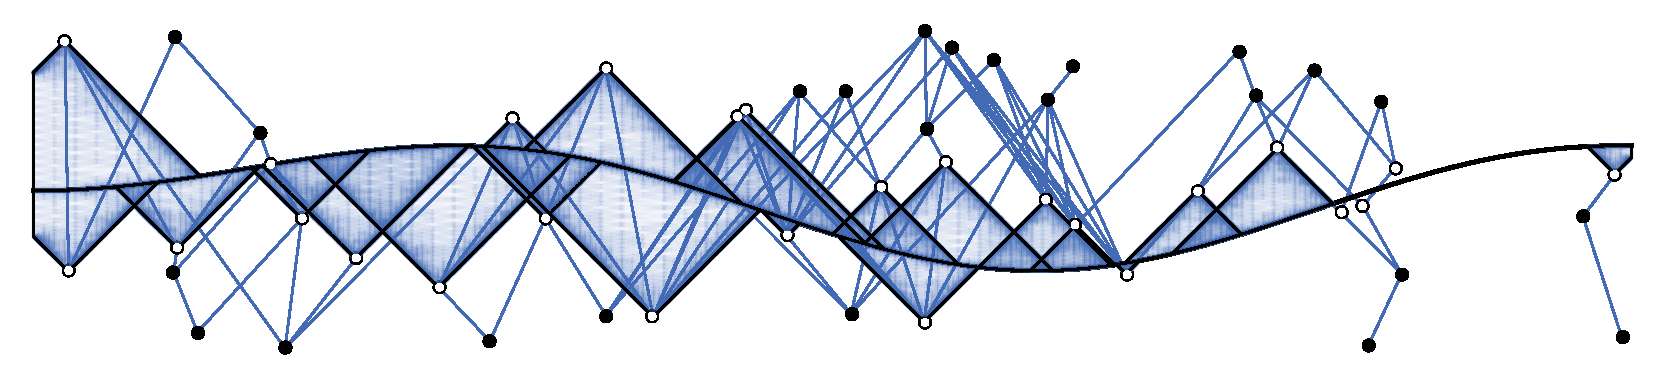
\includegraphics[width=\textwidth]{minmaxplot}}
     \caption{An illustration of the idea. Pictured here is a causal set obtained by a sprinkling into a spacetime partitioned by a spacelike hypersurface. The minimal and maximal points about the surface are highlighted and the shaded regions illustrate the regions whose volumes $V_\blacktriangle$ and $V_\blacktriangledown$ are needed in the proof.}
     \label{fig:Nmin_Nmax}
\end{figure}

\section{The Proof}

\subsection{Poisson Sprinklings for $\langle N_{max}\rangle$ and $\langle N_{min}\rangle$}

In order to prove~\eqref{eq:mainconjecture} let us first derive an expression for the mean value of $S^{(d)}_{GHY}[\mathcal C]$. For any instance of the sprinkling, the probability that a sprinkled point $p\in M$ below the surface $\Sigma$ is \emph{maximal} is given by the probability that no point of the sprinkling lies in the region $J^{+}(p)\cap J^{-}(\Sigma)$, the intersection of the causal future of $p$ with the causal past of the surface $\Sigma$.\footnote{For notational convenience we use the symbol $x$ to refer to the causal element $x\in\mathcal C$, to its embedding in the manifold $M$, and to its coordinates in some chart on $M$.} This region will in general be the interior of some curvy $d$-dimensional cone truncated by the surface $\Sigma$, as illustrated in Figure~\ref{fig:Nmin_Nmax}. We will refer to these regions as \emph{truncated cones} below. The Poisson process assigns a probability
\be\label{Poisson}
\mathbb P\left(\text{no points in }J^{+}(p)\cap J^{-}(\Sigma)\right)=e^{-\rho V_\blacktriangledown(p)}
\ee
to this event, where $V_\blacktriangledown(p)\equiv V(J^{+}(p)\cap J^{-}(\Sigma))$ is the spacetime volume of the region $J^{+}(p)\cap J^{-}(\Sigma)$. The probability of sprinkling an element into an infinitesimal four-volume $dV_p$ at $p$ is $\rho dV_p$ where $\rho=l^{-d}$ is the sprinkling density, and so the total expected number of maximal elements below $\Sigma$ is
\be\label{eq:nmax}
\left\langle N_{max}\right\rangle =\rho\int_{J^{-}(\Sigma)}dV_p\; e^{-\rho V_\blacktriangledown(p)}
\ee
Similarly the expected number of minimal elements above $\Sigma$ is
\be\label{eq:nmin}
\left\langle N_{min}\right\rangle =\rho\int_{J^{+}(\Sigma)}dV_p\; e^{-\rho V_\blacktriangle(p)}
\ee
where $V_\blacktriangle(p)\equiv V(J^{+}(\Sigma)\cap J^{-}(p))$.

In the limit $\rho\rightarrow\infty$, both quantities will diverge, but if their difference $\langle N_{max}\rangle - \langle N_{min}\rangle = \langle N_{max} - N_{min}\rangle$ grows slower than or at order $\rho^{1-\frac2d}$, the proposed action~\eqref{GH_boundary_to_causet} will tend to a finite value in the continuum limit.

Consider a set of synchronous or Gaussian Normal Coordinates (GNC) $x^\mu=(t,\mathbf x)$ adapted to $\Sigma$ such that in a neighbourhood $U_\Sigma$ of $\Sigma$ the line element is
\be
ds^2 = -dt^2 + h_{ij}(t,\mathbf x) dx^i dx^j.
\ee
In these coordinates, the surface $\Sigma$ corresponds to $t=0$, and the coordinate $t$ measures the proper time elapsed along geodesics whose tangent vector is proportional to the surface normal on $\Sigma$.
%\be\label{GNC_metric}
%g_{\mu\nu}(x)=
%\begin{pmatrix}
 %-1&0 \\
% 0&h_{ij}(x)
%\end{pmatrix}.
%\ee
%In order to find $N_{max}$, the number of maximal points below the surface, one has to use the fact that the points have been sprinkled with a Poisson distribution. 
%If we pick a point $x_0=(0,\mathbf{x})\in \Sigma$ on the surface that has the same spatial coordinates as $x=(t,\mathbf{x})$ then the coordinate time, $t$, is the proper time elapsed along the unique geodesic between $x_0$ and $x$. The volume $V(\Sigma,x)$ then only depends on $t$.~\mb{error?}  
The integrals~\eqref{eq:nmax} and ~\eqref{eq:nmin} seem intractable as they stand, since the integration is over the entire causal past/future of the surface and the volume expressions will be complicated in the presence of curvature. However, for large $\rho$ (small $l$), the integrands $\exp(-\rho V)$ will be exponentially suppressed unless the volumes are small. Consider the spacetime region $U_\epsilon=\left\{|t|<\epsilon\right\}$ around the surface $\Sigma$ for some $\epsilon>0$ (with $\epsilon$ small enough such that the GNC system is valid throughout $U_\epsilon$). We will assume that for any such $\epsilon$, the contribution from points with $|t|>\epsilon$ to the integrals~\eqref{eq:nmax} and \eqref{eq:nmin} can be made arbitrarily small by setting $\rho$ large enough, since the volumes of the truncated past/future lightcones for such points will be too large. Hence, as $\rho\rightarrow\infty$, the integration ranges in \eqref{eq:nmax} and \eqref{eq:nmin} can be cut off at finite time $t=\pm\epsilon$ with $\epsilon$ arbitrarily small, which allows us to expand the time integration-variable about zero. These assumptions of course impose certain regularity conditions on the surface $\Sigma$, but we will assume that they are reasonable conditions.\mb{say more about this? we can't have an asymptotically null surface i suppose} The integrals then simplify to

\begin{align}\label{eq:nmax_and_eq:nmin}
\left\langle N_{max}\right\rangle & =\int_{\Sigma}d^{d-1}x\int_{-\varepsilon}^{0}dt\:
h^{\frac{1}{2}}\left(1+
\frac{1}{2}\frac{\dot{h}}{h}t+O(t^2)\right)
 \rho\ e^{-\rho V_\blacktriangledown(t,\mathbf x)}
\\
\left\langle N_{min}\right\rangle & =\int_{\Sigma}d^{d-1}x\int_{0}^{\varepsilon}dt\:
h^{\frac{1}{2}}\left(1+
\frac{1}{2}\frac{\dot{h}}{h}t+O(t^2)\right) \rho\ e^{-\rho V_\blacktriangle(t,\mathbf x)}
\end{align}
where $h\equiv det\left(h_{ij}(0,\mathbf{x})\right)$ and $\dot{}\equiv \frac{\partial}{\partial t}$ and the metric determinant has been in expanded in small $t$.

The only truncated cones that contribute will have small volumes, as we are restricting ourselves close to the surface.\mb{this sounds circular w.r.t. last paragraph} This means that the volumes can be approximated by the volumes of less curvy cones, and it can be shown that higher order corrections, in the approximation scheme, vanish in the limit of $\rho \rightarrow \infty$. This will all be made more precise below. The approximation procedure will be outlined below for a cone to the future of $\Sigma$, as the process for the past cone is nearly identical.

\subsection{Lightcone Volumes}

In order to evaluate the volume $V_\blacktriangledown(p)$ or $V_\blacktriangle(p)$ of a truncated cone we will perform a coordinate transform to Riemann Normal Coordinates (RNCs) in a neighbourhood containing the cone. The discussion for the two volume integrals is identical so we will outline that for $V_\blacktriangle(p)$ (i.e. for points to the future of $\Sigma$). 

Fix $p\in M$ and denote its coordinate values in GNCs by $x^\mu_p=(t_p,\mathbf x_p)$. It will be convenient to use RNCs centered not at the tip $p$ of the cone but instead at the point $p_0$ where the unique geodesic through $p$ whose tangent is normal to $\Sigma$ intersects $\Sigma$. In GNCs this simply corresponds to the point $p_0$ with coordinates $x_0^\mu=x^\mu(p_0)=(0,\mathbf x_p)$. RNCs centered at $p_0$ will be given the symbol $y^{\overline{\mu}}$.
\mb{let's put all facts about $x^\mu$ and $y^{\overline\mu}$ for $p$ and $p_0$ here and expansion of det in RNC.} We need to assume that for any $p$ in $U_\epsilon$, the Riemann normal neighbourhood $U_p\subset M$ (throughout which the RNC system centered at $p_0$ is well-defined) contains the truncated cone $J^-(p)\cap J^+(\Sigma)$. This assumption seems reasonable given the that $U_\epsilon$ can be made arbitrarily ``thin'' as $\rho\rightarrow\infty$. In RNCs the metric and the Christoffel symbols at $p_0$ are those of flat space:
\be\label{eq:RNCMetricTransAtPAndChris}
g_{\overline{\mu} \overline{\nu}}(p_0)=\eta_{\overline{\mu} \overline{\nu}}=A^{\mu}_{\;\overline{\mu}}A^{\nu}_{\;\overline{\nu}}g_{\mu\nu}(p_0)\;,\;\;\;\;\Gamma^{\overline{\mu}}_{\;\overline{\nu}\overline{\rho}}(p_0)=0
\ee
The $A^{\mu}_{\;\overline{\mu}}$ govern the coordinate transformation from GNCs to RNCs to linear order. %but $O(x^2)$ corrections may be required. 
To second order the coordinate transformation is given by
\be\label{eq:RNCtotaltrans}
y^{\overline{\mu}}=A^{\overline{\mu}}_{\;\nu}x^\nu+\frac{1}{2}A^{\overline{\mu}}_{\;\mu}\Gamma^{\mu}_{\;\nu\rho}(p_0)x^\nu x^\rho+O((x-x_0)^3).
\ee
The inverse relation to first order is 
\be\label{eq:RNCinversetrans}
x^{\mu}=A^{\mu}_{\;\overline{\nu}}y^{\overline{\nu}}+O(y^2)
\ee
and one finds that the $A^{\mu}_{\;\overline{\mu}}$ satisfy
\be\label{eq:RNCeqnforA}
A^{\overline{\mu}}_{\;\mu}A^{\mu}_{\;\overline{\nu}}=\delta^{\overline{\mu}}_{\;\overline{\nu}}\;,\;\;\;\;A^{\mu}_{\;\overline{\mu}}A^{\overline{\mu}}_{\;\nu}=\delta^{\mu}_{\;\nu}
\ee
These relations for RNC will cover all that will be needed in this discussion.

Now the volume of the truncated cone can be found as follows. 
%Consider the past lightcone emanating at the point $p_0=(T,\mathbf x_0)$ truncated by $\Sigma$. There is a unique point $q_0=(0,\mathbf x_0)$ on $\Sigma$ associated with $p_0$, separated from $p_0$ by proper time $T$. 
The volume of the cone is given by

\be\label{eq:VolumeWithNoSimplifications}
V_\blacktriangle(p)=\int_{\mathcal{X}_p} d^d x\;\sqrt{-g}
\ee
where the integration region, $\mathcal{X}_p\equiv  J^-(p)\cap J^+(\Sigma)$ will be a complicated expression. As we are dealing with points close to the surface we can use the  RNCs $y^{\overline{\mu}}$, defined as above, about the point $p_0$. Let us denote the time-coordinate of $p$ in GNCs by $T=x^0_p=t_p$. For the transformation from GNCs to RNCs at $p_0$ one finds that $A^{\overline 0}_{\;0}=1$, $A^{\overline 0}_{\;i}=0$ and $\delta_{\ibar\jbar}=A^i_{\;\ibar}A^j_{\;\jbar}h_{ij}(p_0)$, which in particular implies $y^{\overline{0}}_p=\overline{t}_p=t_p=T$. \mb{more detail needed i think}It can then be shown that the volume integral reduces to~\cite{Khetrapal_Sumati:Causal_Diamond_Volume}

\be\label{eq:VolumeWithRNC}
V_\blacktriangle(p) =\int_{\mathcal{X}}d^dy+\int_{\mathcal{X}_0}d^dy\left(-\frac{1}{6}R_{\overline{\mu}\overline{\nu}}(p_0)y^{\overline{\mu}}y^{\overline{\nu}} \right)+O(T^{d+3})
\ee
where $\mathcal{X}_0=\left\lbrace y^{\overline{\mu}} \mid 0 \leq \overline{t}\leq T\; ,\; (y^{\overline{1}})^2+(y^{\overline{2}})^2+...+(y^{\overline{d-1}})^2\leq (T-\overline{t})^2 \right\rbrace$ is what we call the \textit{flat cone}, and $R_{\overline{\mu}\overline{\nu}}(p_0)$ is the Ricci tensor in RNC evaluated at $p_0$.\mb{justify beforehand which orders to keep?}
%The arguments of the volume function need not be changed as the volume only depends on the points in the manifold, $q_0$ and $p_0$. 
The flat cone term comes in at $O(T^{d+2})$ so the volume we have to calculate has reduced to

\be\label{eq:VolumeToLowestOrder}
V_\blacktriangle(p) =\int_{\mathcal{X}}d^dy+O(T^{d+2})
\ee
Terms of $O(T^{d+2})$ can be retained till the end, but in the limit, $\rho\rightarrow\infty$, they vanish. This will be proved below.

This is now a simple volume integral but we need to find the boundaries of $\mathcal{X}$ for the correct integration limits. There are two boundaries to the (solid) truncated cone: the lightcone emanating at $p$ and the base, given by the intersection of $\Sigma$ with the interior of the lightcone. First we look at the lightcone. Following \cite{Khetrapal_Sumati:Causal_Diamond_Volume} it can be shown that the first curvature correction to the lightcone comes in at $O(T^{d+2})$ and so can be ignored for our purposes. This means that the lightcone can be treated as effectively flat in RNCs and thus corresponding to the set $(y^{\overline{1}})^2+(y^{\overline{2}})^2+...+(y^{\overline{d-1}})^2= T-\overline{t}$.\mb{what limit on $\bar t$?}

The base of the cone in GNCs is simply a part of the surface $t=0$, so we can use (\ref{eq:RNCtotaltrans}) to find the equation for the surface in RNCs. Equation (\ref{eq:RNCtotaltrans}) gives

\be\label{eq:BottomSurfaceWithGNC}
\overline{t}=\frac{1}{2}\Gamma^{0}_{\;ij}(p_0)x^i x^j+O( x^3)\ee

The first part on the right of (\ref{eq:RNCtotaltrans}) vanishes as $A^{\overline{0}}_{\;\mu}x^{\mu}=x^0$ (as $A^{\overline{0}}_{\;i}=0$ and $A^{\overline{0}}_{\;0}=1$) and $x^0=t=0$ for the bottom surface. Using the inverse RNC relation (\ref{eq:RNCinversetrans}) one can find the equation for the bottom surface in RNCs:

\be\label{eq:BottomSurface}
\overline{t}=\frac{1}{2}\Gamma^{0}_{\;ij}(p_0)A^{i}_{\;\ibar}A^{j}_{\;\jbar}y^{\ibar} y^{\jbar}+O(y^3)
\ee

Let us rewrite this equation in spherically symmetric coordinates, i.e. define $r=\sqrt{\delta_{\ibar\jbar}y^\ibar y^\jbar}$ and the usual angular coordinates $\phi_1,..,\phi_{d-2}$ in terms of the spatial coordinates $y^{\overline{1}} = r \cos(\phi_1),\ldots, y^{\overline{d-1}} = r \sin(\phi_1) \cdots \sin(\phi_{d-3}) \sin(\phi_{d-2})$. Then

\be\label{eq:RadialBottomSurface}
\overline{t}=\frac{1}{2}\left(\Gamma^{0}_{\;ij}(p_0)A^{i}_{\;\ibar}A^{j}_{\;\jbar}\frac{y^{\ibar} y^{\jbar}}{r^2}\right)r^2+O(y^3)=\frac{1}{2}f(\mathbf{x}_p,{\boldsymbol\phi})r^2+O(y^3)
\ee
where $\boldsymbol\phi$ stands collectively for all the angular coordinates $\phi_1,..,\phi_{d-2}$. The function $f(\mathbf{x}_p,\boldsymbol\phi)$ depends on $\mathbf{x}_p$ since $\Gamma^{0}_{\;ij}$ and $A^{i}_{\;\ibar}$ depend on $p_0$.
%One can see that $f(\mathbf{x}_0,\boldsymbol\phi)$ depends on the angles, $\phi$, by substituting the relations below into (\ref{eq:RadialBottomSurface})
%\begin{equation}
%\begin{aligned}\label{eq:SphericalCoords}
%y^{\overline{1}} &= r \cos(\phi_1)  \\
%y^{\overline{2}} &= r \sin(\phi_1) \cos(\phi_2)  \\
%y^{\overline{2}} &= r \sin(\phi_1) \sin(\phi_2) \cos(\phi_3)  \\
%    &\vdots  \\
%y^{\overline{d-2}} &= r \sin(\phi_1) \cdots \sin(\phi_{d-3}) \cos(\phi_{d-2})  \\
%y^{\overline{d-1}} &= r \sin(\phi_1) \cdots \sin(\phi_{d-3}) \sin(\phi_{d-2})
%\end{aligned}
%\end{equation}

With the boundaries of the integration region in place, we can now write down the integral explicitly in spherical coordinates:

\be\label{eq:VolumeIntegralSpherical}
V_\blacktriangle(p)=\int_{S^{d-2}}
d\Omega_{d-2}
\int_{0}^{r_{max}(\phi)}r^{d-2}dr
\int_{\frac{1}{2}f(\mathbf{x}_p,\phi)r^2}^{-r+T}
d\overline{t}+O(T^{d+2})
\ee
where $r_{max}(\boldsymbol\phi)$ is the value of the radial coordinate for which the surface $\Sigma$ intersects the lightcone at angle $\boldsymbol\phi$, as shown in Figure \ref{fig:cone_plot}. To find this value one needs to solve 
\be
\frac{1}{2}f(\mathbf{x}_p,\boldsymbol\phi){r_{max}}^2(\boldsymbol\phi)=-r_{max}(\boldsymbol\phi)+T
\ee 
for $r_{max}(\boldsymbol\phi)$ and take the positive solution. The solution can be expanded in $T$ and is simply $r_{max}=T+O(T^2)$, with angular dependent terms contributing at $O(T^2)$. The $O(T^2)$ term will contribute at $O(T^{d+2})$ in the integral and so can be ignored. Substituting $r_{max}=T$ into (\ref{eq:VolumeIntegralSpherical}) lets us evaluate the integral and we find 
\begin{figure}[t]
  \centering
    {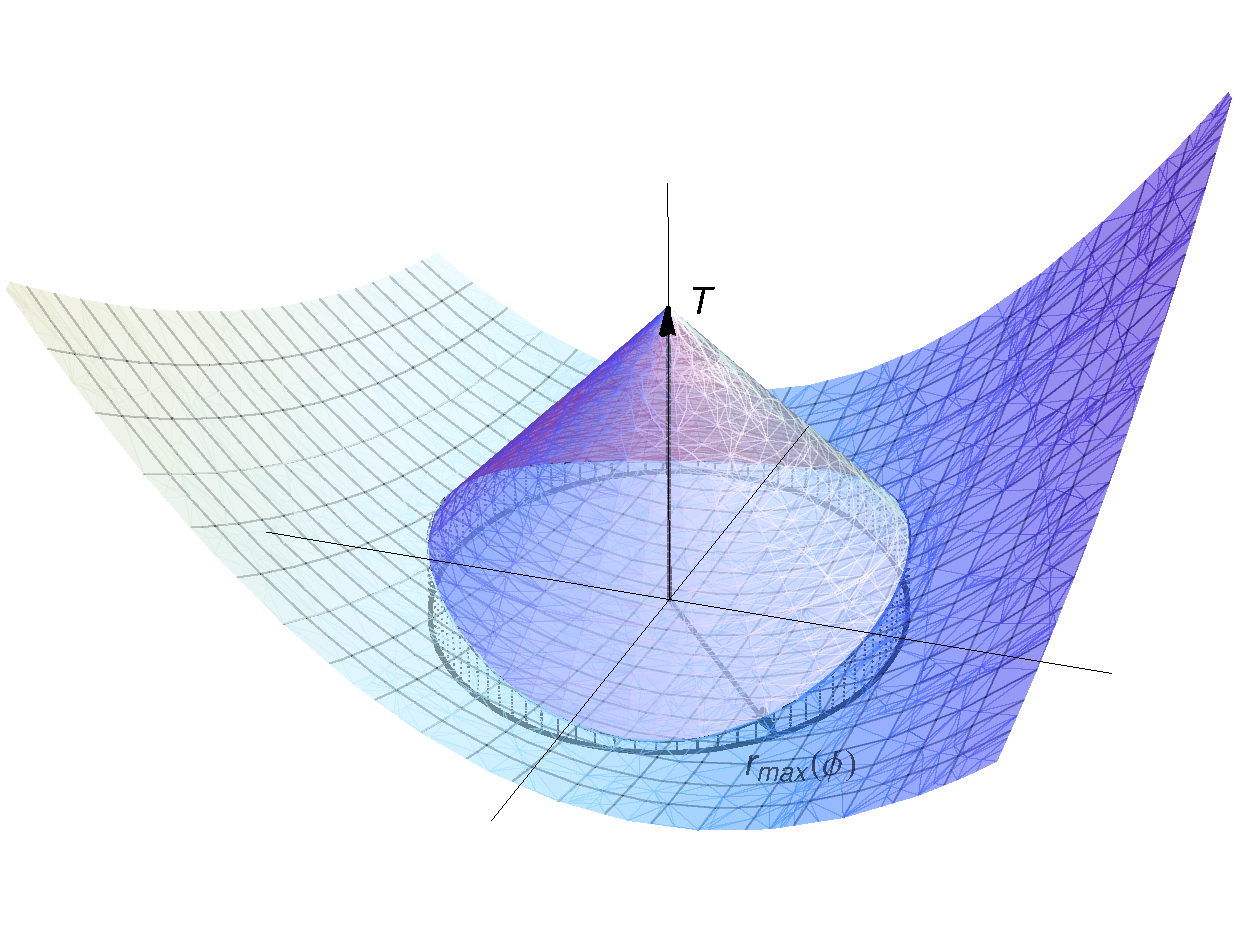
\includegraphics[scale=0.5]{coneplot}}
     \caption{The size of the region inside the top and bottom bounding surfaces is the volume we want to calculate.}
     \label{fig:cone_plot}
\end{figure}
\be\label{eq:VolumeNoK}
V_\blacktriangle(p)
=\frac{A_{d-2}}{d(d-1)}T^d\left(1-\frac{d}{2(d+1)}\Gamma^{0}_{\;ij}(p_0)A^{i}_{\;\ibar}A^{j}_{\;\jbar}\delta^{\ibar\jbar}T\right)
+O(T^{d+2})
\ee
where $A_{d-2}$ is the volume of the unit $(d-2)$-sphere and the $\delta^{\ibar\jbar}$ comes from the fact that cross terms ($\ibar\neq \jbar$) vanish under the angular integration. The defining relations for $A^{i}_{\;\ibar}$ can now be rearranged to give $A^{i}_{\;\ibar}A^{j}_{\;\jbar}\delta^{\ibar\jbar}=h^{ij}(p_0)$. Now in GNCs the extrinsic curvature on the surface is given by
\be\label{eq:K}
K
=g^{\mu\nu }\nabla_{\mu}n_{\nu}
=-\Gamma^{0}_{\;ij}h^{ij}=-\frac{1}{2}\frac{\dot{h}}{h}.
\ee
Substituting this into~\eqref{eq:VolumeNoK} with we obtain 
\begin{align}
V_\blacktriangle(T,\mathbf x)
&=\frac{A_{d-2}}{d(d-1)}T^d\left(1+\frac{d}{2(d+1)}K(0,\mathbf{x})T\right)
+O(T^{d+2}) \label{eq:TopVolumeWithK}\\
V_\blacktriangledown(-T,\mathbf x)
&=\frac{A_{d-2}}{d(d-1)}T^d\left(1-\frac{d}{2(d+1)}K(0,\mathbf{x})T\right)
+O(T^{d+2}), \label{eq:BottomVolumeWithK}
\end{align}
having dropped the subscript $p$. Given the volume expressions in GNCs we now proceed to evaluate the integrals for $\langle N_{min}\rangle $ and $\langle N_{max}\rangle$.

\subsection{The mean of $S^{(d)}_{GHY}[\mathcal C]$}

Using the previous equation we obtain for (\ref{GH_boundary_to_causet}) in the limit $\rho \rightarrow \infty$
\begin{gather}\label{eq:NmaxNminStart}
\begin{aligned}
\lim_{\rho \to \infty}\rho^{\frac{2}{d}-1}\left\langle N_{max}-N_{min} \right\rangle &= \\
\lim_{\rho \to \infty}\rho^{\frac{2}{d}}
\int_{\Sigma}d^{d-1}x & \int_{-\varepsilon}^{0}dt\
h^{\frac{1}{2}}\left(1+
\frac{1}{2}\frac{\dot{h}}{h}t+\rho B(-t)^{d+1}+\rho O(t^{d+2})\right)e^{-\rho A(-t)^{d}} \\
-\rho^{\frac{2}{d}}\int_{\Sigma}d^{d-1}x &
\int_{0}^{\varepsilon}dt\
h^{\frac{1}{2}}\left(1+
\frac{1}{2}\frac{\dot{h}}{h}t-\rho Bt^{d+1}+\rho O(t^{d+2})\right)e^{-\rho At^{d}}
\end{aligned}
\end{gather}
where we have defined
\begin{gather}\label{A_and_B_defn}
\begin{aligned}
A & \equiv \frac{A_{d-2}}{d(d-1)} \\
B & \equiv \frac{A_{d-2}}{2(d-1)(d+1)}K(0,\mathbf{x})
\end{aligned}
\end{gather}
and we have Taylor expanded the $O(t^{d+1})$ parts of the volume functions, in small $t$, from the exponents. The pre-factor $\rho^{\frac{2}{d}-1}$ accounts for the factors of $l$ in (\ref{GH_boundary_to_causet}). With this pre-factor the limit of the above equation is well defined. Swapping the integration variable to $t\rightarrow -t$ in the first term and combining the two integrals we obtain
\be\label{eq:NmaxNminSimplified}
\lim_{\rho \to \infty}\rho^{\frac{2}{d}}
\int_{\Sigma}d^{d-1}x \int_{0}^{\varepsilon}dt\
h^{\frac{1}{2}}\left(-\frac{\dot{h}}{h}t+2\rho B t^{d+1}+\rho O(t^{d+2}) \right)e^{-\rho At^{d}}
\ee
We now show that $O(t^{d+2})$ and higher terms vanish as $\rho \rightarrow\infty$. All corrections that we have ignored so far contribute at $O(t^{d+2})$ or higher, so proving that these contributions vanish proves that our approximations are justified. Inspecting (\ref{eq:NmaxNminSimplified}) we see that all we need to show is that for integer $n>1$,  the following integral vanishes:

\be\label{eq:VanishingOrderIntegral}
\lim_{\rho \to \infty}\rho^{\frac{2}{d}+1}\int_{0}^{\varepsilon}dt\
t^{d+n}e^{-\rho At^{d}}.
\ee
The additional factor of $\rho$ has come from inside the integral in (\ref{eq:NmaxNminSimplified}). We make the substitution $z=\rho At^{d}$ and find that (\ref{eq:VanishingOrderIntegral}) is proportional to

\be\label{eq:GammaVanishingOrderIntegral}
\lim_{\rho \to \infty}\rho^{\frac{1-n}{d}}\int_{0}^{\rho A\varepsilon^d}dz\;z^{\frac{n+1}{d}}e^{-z}=\lim_{\rho \to \infty}\rho^{\frac{1-n}{d}}\int_{0}^{\infty}dz\;z^{\left[\left(\frac{n+1}{d}+1\right)-1 \right]}e^{-z}
\ee
where $\rho$ has been taken to $\infty$ in the limits on the RHS, and the power of $z$ has been written in this way so that the integral is in the form of a gamma function, $\Gamma(t)=\int_{0}^{\infty}z^{t-1}e^{-z}dz$. Using $\Gamma(t+1)=t\Gamma(t)$ we find that (\ref{eq:GammaVanishingOrderIntegral}) is proportional to
\be\label{eq:GammaVanishingOrder}
\lim_{\rho \to \infty}\rho^{\frac{1-n}{d}}\Gamma\left(\frac{n+1}{d}\right)
\ee
One can see from above that if $n>1$ then this term will vanish, thus proving that terms of $O(t^{d+2})$ or higher will go to $0$ in the limit $\rho\rightarrow\infty$.

The non-vanishing terms of (\ref{eq:NmaxNminSimplified}) can also be put into the form of gamma functions. This allows the integral over $t$ to be evaluated in (\ref{eq:NmaxNminSimplified}). One also sees that we have terms like $\frac{\dot{h}}{h}$, and from (\ref{eq:K}) we know that these can be written in terms of the extrinsic curvature $K$. We find then that (\ref{eq:NmaxNminSimplified}) reduces to

\be\label{eq:nmax_eq:nmin_end}
\lim_{\rho \to \infty}\rho^{\frac{2}{d}-1}\left\langle N_{max}-N_{min} \right\rangle=
\frac{2(d+2)}{d(d+1)}
\left[\frac{A_{d-2}}{d(d-1)}\right]^{-\frac{2}{d}}
\Gamma\left(\frac{2}{d}\right)\int_{\Sigma}d^{d-1}x\
\sqrt{h}K(0,\mathbf{x}).
\ee
$K(0,\mathbf{x})$ is evaluated at the surface and is therefore the same $K$ as in equation (\ref{GH_boundary_to_causet}). We can therefore conclude that to make (\ref{eq:mainconjecture}) true we need a factor $l_{p}^{2-d}$ to make our expression dimensionless, and a value of $c_d$ equal to that of equation (\ref{Cn}). This concludes the proof of the conjectured equality in (\ref{eq:mainconjecture}).

\section{Fluctuations}
So far we have only talked about the mean of the causal set boundary action. Let us now turn to its fluctuations (its standard deviation) $\sigma[S^{(d)}_{GHY}(\mathcal C)]=\text{Var}[S^{(d)}_{GHY}(\mathcal C)]^\frac12$.\footnote{Whenever we say fluctuations we refer to the standard deviation of the random variable, not to its variance.} We can make a heuristic argument to estimate the dependence of fluctuations on $\rho=l^{-d}$. In any spacetime region of fixed volume $V$ the number of causal set elements $N$ experiences Poisson fluctuations of order $\sqrt N$. Since $N_{max}$ and $N_{min}$ are quantities associated with a codimension-1 surface (counting elements ``near" $\Sigma$), we may expect them to inherit fluctuations of order $N^\frac{d-1}{2d}$. Then the action $S^{(d)}_{GHY}$, being proportional to $\rho^\frac{d-2}{d}$ times the difference of two independent\footnote{The independence is as a feature of the Poisson process in $M$: the number of elements $N(R)$ in any subregion $R\subset M$ is a Poisson variable itself, and for any two disjoint regions $R_1$, $R_2$ the numbers $N(R_1)$ and $N(R_2)$ are independent random variables.} random variables with standard deviation $N^\frac{d-1}{2d} = (\rho V)^\frac{d-1}{2d}$ should see fluctuations of order $\rho^\frac{2-d}{d}\rho^\frac{d-1}{2d}=\rho^\frac{d-3}{2d}$. This suggests that for $d=2$ these fluctuations should grow as $\rho\rightarrow\infty$, for $d=3$ they should be constant, and for $d>3$ they should be damped.

In order to test this heuristic argument one may like to write down the integral expression for $\text{Var}[S^{(d)}_{GHY}(\mathcal C)]^\frac12$ but it is complicated enough even in finite regions of flat space that it is not very illuminating to reproduce it here. It also seems far less tractable than the expression for the mean because it involves terms of the type $\int d^dx\int d^dy \exp\left[-\rho V(J^+(x)\cap J^+(y))\right]$ for which the above methods of cutting off the time-integration range and Taylor expanding will not follow through. Instead we will show the results of computer simulations that support results of the heuristic argument. 
 
The simulations were carried out as follows. Denote the discreteness scale by $l$. Take a $d$-cube $[0,L]^d$ in $d$-dimensional Minkowski space with metric $ds^2=-dt^2+d{\mathbf x}^2$ and define the hypersurface $\Sigma: t=L/2$, which partitions the cube into two halves. Sprinkle at density $\rho=l^{-d}$ into the cube, which in any given run will place $N$ points inside the cube where $N$ is a Poisson random number with mean $\left\langle N\right\rangle = \rho V=  (L/l)^d$. Evaluate $S^{(d)}_{GHY}=c_d\rho^\frac{d-2}{d}(N_{min} - N_{max})$ for $\Sigma$ by counting the minimal/maximal elements in the upper/lower half of the cube, and repeat for $R$ runs.

\newpage

\bibliographystyle{jhep}

\bibliography{references}

\end{document}


%%
JHEPPUB:

\title{Gibbons-Hawking-York Boundary Term in Causal Sets}
 \author[a]{M. Buck}
 \author[a,b]{\!, F. Dowker}
 \author[a]{and I. Jubb\,}
\affiliation[a]{Theoretical Physics Group, Blackett Laboratory, Imperial College, London, SW7 2AZ, U.K.}
\affiliation[b]{Institute for Quantum Computing, University of Waterloggedo, ON, N2L 2Y5, Canada}

\abstract{ 
We show some stuff.
}

\begin{document}

\maketitle

\pagebreak

\noindent NOTES:\\
1. define s as the RV, not as its mean

\section{Introduction}




%%IOPART

\begin{document}

\title{Gibbons-Hawking-York Boundary Term in Causal Sets}

\author{Michel Buck Fay Dowker, Ian Jubb}
\address{Blackett Laboratory, Imperial College, London, SW7 2AZ, U.K.}

\begin{abstract}

We show some stuff.

\end{abstract}
%\pacs{03.67.-a, 03.65.Ta, 03.70.+k}

\maketitle
\section{Introduction}
%%